\documentclass[norsk,a4paper,11pt]{article}
\usepackage[T1]{fontenc} %for å bruke æøå
\usepackage[utf8]{inputenc}
\usepackage{amsmath, amsfonts, amssymb}
\usepackage{graphicx} %for å inkludere grafikk
\usepackage{verbatim} %for å inkludere filer med tegn LaTeX ikke liker
\usepackage[font=scriptsize]{caption}
\usepackage{subcaption}
\usepackage{mdwlist}
\usepackage{bm}
\usepackage{enumerate}
\usepackage[usenames, dvipsnames]{color}
%\usepackage{hyperref}
\usepackage{url}
% By default the URLs are put in typewriter type in the body and the
% bibliography of the document when using the \url command.  If you are
% using many long URLs you may want to uncommennt the next line so they
% are typeset a little smaller.
% \renewcommand{\UrlFont}{\small\tt}
\newcommand*\diff{\mathop{}\!\mathrm{d}}
\def\mbf#1{\mathbf{#1}}
\newcommand{\VV}{\mathbf{V}}
\newcommand{\Vv}{\mathbf{v}}
\newcommand{\VX}{\mathbf{X}}
\newcommand{\Vx}{\mathbf{x}}
\newcommand{\VH}{\mathbf{H}}
\newcommand{\Vh}{\mathbf{h}}
\newcommand{\VW}{\mathbf{W}}
\newcommand{\Vwi}{\mathbf{w}_{i*}}
\newcommand{\Vwj}{\mathbf{w}_{*j}}
\newcommand{\Va}{\mathbf{a}}
\newcommand{\Vb}{\mathbf{b}}

\bibliographystyle{plain}


\title{The Restricted Boltzmann Machine}

\begin{document}
\date{\today}
\maketitle


\section{Introduction}
\begin{itemize}
	\item Why use a generative ("dreaming") model rather than the more well known discirminative deep neural networks (DNN)? 
	\begin{itemize}
		\item Discriminitave methods have several limitations: They are supervised learning methods, thus requiring labeled data. And there are tasks they cannot accpomlish, like drawing new examples from an unknown probability distribution.
		\item A generative model can learn to represent and sample from a probability distribution. The core idea is to learn a parametric model of the probability distribution from which the training data was drawn. Fex: 
		\begin{itemize}
			\item A model for images could learn to draw new examples of cats and dogs, given a training dataset of images of cats and dogs.
			\item Generate a sample of an ordered or disordered Ising model phase, having been given samples of such phases.
		\end{itemize}
	\end{itemize}
	\item Some similarities and differences from DNNs:
	\begin{itemize}
		\item Both use gradient-descent based learning procedures for minimizing cost functions
		\item Energy based models don't use backpropagation and automatic differentiation for computing gradients, instead turning to Markov Chain Monte Carlo methods.
		\item DNNs often have several hidden layers. A restricted Boltzmann machine has only one hidden layer, however several RBMs can be stacked to make up Deep Belief Networks, of which they constitute the building blocks.
	\end{itemize}
	\item History: The RBM was developed by amongst others Geoffrey Hinton, called by some the "Godfather of Deep Learning", working with the University of Toronto and Google.
\end{itemize}


\section{The Restricted Boltzmann machine}
\subsection{Structure}

\begin{figure}
    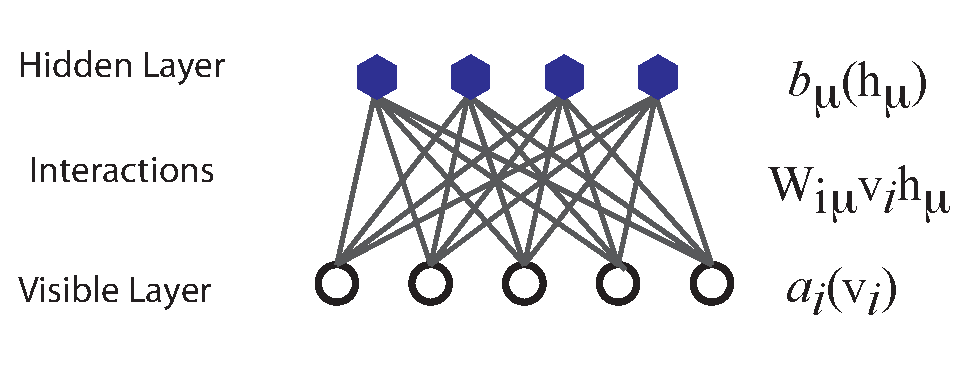
\includegraphics[width=0.9\linewidth]{RBM.pdf}
    \caption{
        \label{fig:RBMgraph}
        The RBM graph}
\end{figure}


See figure \ref{fig:RBMgraph} to see the structure of the RBM graph. We here see some of the essential components of the restricted Boltzmann machine:
\begin{itemize}
\item The network layers:
\begin{itemize}
	\item $\Vx$ represents the visible layer, a vector of $M$ elements (nodes). This layer represents both what the RBM might be given as training input, \textit{and} what we want it to be able to reconstruct. This might for example be the pixels of an image, the spin values of the Ising model, or coefficients representing speech.
	\item $\Vh$ represents the hidden, or latent, layer. A vector of $N$ elements (nodes). Also called "feature detectors".
\end{itemize}
The goal of the hidden layer is to increase the model's expressive power. We encode complex interactions between visible variables by introducing additional, hidden variables that interact with visible degrees of freedom in a simple manner, yet still reproduce the complex correlations between visible degrees in the data once marginalized over (integrated out).

Examples of this trick being employed in physics: 
\begin{itemize}
	\item The Hubbard-Stratonovich transformation
	\item The introduction of ghost fields in gauge theory
\end{itemize}

\item The network parameters, to be optimized/learned:
\begin{itemize}
		\item $\Va$ represents the visible bias, a vector of same lenght as $\Vx$.
		\item $\Vb$ represents the hidden bias, a vector of same lenght as $\Vh$.
		\item $W$ represents the interaction weights, a matrix of size $M\times N$.
\end{itemize}
\end{itemize}


\subsection{Joint distribution and the Energy function}
The restricted Boltzmann machine is described by a Bolztmann distribution

\begin{align}
	P_{rbm}(\Vx,\mathbf{h}) = \frac{1}{Z} e^{-\frac{1}{T_0}E(\Vx,\mathbf{h})}
\end{align}
where $Z$ is the normalization constant or partition function, defined as 
\begin{align}
	Z = \int \int e^{-\frac{1}{T_0}E(\Vx,\mathbf{h})} \diff \Vx \diff \mathbf{h}
\end{align}

It is common to ignore $T_0$ by setting it to one. 

The function $E(\Vx,\mathbf{h})$ gives the \textit{energy} of a configuration (pair of vectors) $(\Vx, \Vh)$. The lower the energy of a configuration, the higher the probability of it. This function also depends on the parameters $\Va$, $\Vb$ and $W$. Thus, when we adjust them during the learning procedure, we are adjusting the energy function to best fit our problem.

\subsection{Defining different types of RBMs}
There are different variants of RBMs, and the differences lie in the types of visible and hidden units we choose as well as in the implementation of the energy function $E(\Vx,\mathbf{h})$. 

\subsubsection{Binary-Binary RBM}
RBMs were first developed using binary units in both the visible and hidden layer. The corresponding energy function is defined as follows:

\begin{align}
	E(\Vx, \mathbf{h}) = - \sum_i^M x_i a_i- \sum_j^N b_j h_j - \sum_{i,j}^{M,N} x_i w_{ij} h_j
\end{align}
where the binary values taken on by the nodes are most commonly 0 and 1.

\subsubsection{Gaussian-Binary RBM}
Another varient is the RBM where the visible units are Guassian while the hidden units remain binary:
\begin{align}
	E(\Vx, \mathbf{h}) = \sum_i^M \frac{(x_i - a_i)^2}{2\sigma_i^2} - \sum_j^N b_j h_j - \sum_{i,j}^{M,N} \frac{x_i w_{ij} h_j}{\sigma_i^2} 
\end{align}
\begin{itemize}
	\item Useful when we model continuous data (i.e., we wish $\Vx$ to be continuous)
	\item Requires a smaller learning rate, since there's no upper bound to the value a component might take in the reconstruction
\end{itemize}

\subsubsection{Other RBMs}
Other types of units include:
\begin{itemize}
	\item Softmax and multinomial units
	\item Gaussian visible and hidden units
	\item Binomial units
	\item Rectified linear units
\end{itemize}

\subsection{Sampling}
In order to sample from the RBM probability distribution it is common to use Markov Chain Monte Carlo (MCMC) algorithms such as Metropolis-Hastings or Gibbs sampling.

\subsubsection{Metropolis sampling}
Metropolis sampling starts by suggesting a new configuration $\bm{x}^{k+1}$. In the brute force method this is done by some random change of the visible units. The new configuration is then accepted with the acceptance probability
\begin{align}
	A(\bm{x}^k \rightarrow \bm{x}^{k+1}) = \text{min} (1, \frac{P(\bm{x}^{k+1})}{P(\bm{x}^k)})
\end{align} 

Where we need the marginalized probability
\begin{align}
	P(\bm{x})  &= \sum_\mathbf{h} P_{rbm}(\mathbf{x}, \mathbf{h}) \\
				&= \frac{1}{Z}\sum_\mathbf{h} e^{-E(\mathbf{x}, \mathbf{h})}
\end{align}

\subsubsection{Gibbs sampling}
In this method we sample from the joint probability $P_{rbm} (\Vx, \Vh)$ by way of a two step sampling process. We alternately update the visible and hidden units.
New samples are generated according to the conditional probabilities $P(x_i|\Vh)$ and $P(h_j|\Vx)$ respectively and accepted with the probability of $1$. While the the visible nodes are dependent on the hidden nodes and vice versa, the nodes are independent of other nodes within the same layer. This is due to there being no intra layer interactions in the restricted Boltzmann machine.

The conditional probabilities are often referred to as the activitation functions in the neural networks context due to their role in determining the node outputs. For the binary-binary RBM they are
\begin{align}
	P(h_j = 1 | \bm{x}) &= \frac{1}{1 + e^{-b_j - \sum_i x_i w_{ij}}} \\
	P(x_i = 1 | \bm{h}) &= \frac{1}{1 + e^{-a_j - \sum_j h_j w_{ij}}}
\end{align}
where we recognize the logistic sigmoid function $\sigma (x) = 1/(1+exp(-x))$.
For the Gaussian-Binary RBM the conditional probabilities are
\begin{align}
	P(x_i|\mathbf{h}) &= \mathcal{N}(x_i; a_i+ \sum_j h_j w_{ij}, \sigma^2) \\
	P(h_j=1|\mathbf{x}) &=  \frac{1}{1+e^{-b_j-\frac{1}{\sigma^2} \sum_i x_i w_{ij}}}
\end{align}
while the visible units now follow a normal distribution, we see the hidden units again follow the logistic sigmoid function.

\subsection{Cost function}
When working with a training dataset, the most common training approach is maximizing the log-likelihood of the training data. The log likelihood characterizes the log-probability of generating the observed data using our generative model. Using this method our cost function is chosen as the negative log-likelihood. The learning then consists of trying to find parameters that maximize the probability of the dataset, and is known as Maximum Likelihood Estimation (MLE).
Denoting the parameters as $\bm{\theta} = a_1,...,a_M,b_1,...,b_N,w_{11},...,w_{MN}$, the log-likelihood is given by
\begin{align}
	\mathcal{L}(\{ \theta_i \}) &= \langle \text{log} P_\theta(\bm{x}) \rangle_{data} \\
	&= - \langle E(\bm{x}; \{ \theta_i\}) \rangle_{data} - \text{log} Z(\{ \theta_i\})
\end{align}
where we used that the normalization constant does not depend on the data, $\langle \text{log} Z(\{ \theta_i\}) \rangle = \text{log} Z(\{ \theta_i\})$
Our cost function is the negative log-likelihood, $\mathcal{C}(\{ \theta_i \}) = - \mathcal{L}(\{ \theta_i \})$

\subsection{Optimization / Training}
The training procedure of choice often is Stochastic Gradient Descent (SGD). It consists of a series of iterations where we update the parameters according to the equation
\begin{align}
	\bm{\theta}_{k+1} = \bm{\theta}_k - \eta \nabla \mathcal{C} (\bm{\theta}_k)
\end{align}
at each $k$-th iteration. There are a range of variants of the algorithm which aim at making the learning rate $\eta$ more adaptive so the method might be more efficient while remaining stable.

We now need the gradient of the cost function in order to minimize it. We find that
\begin{align}
	\frac{\partial \mathcal{C}(\{ \theta_i\})}{\partial \theta_i}
	&= \langle \frac{\partial E(\bm{x}; \theta_i)}{\partial \theta_i} \rangle_{data}
	+ \frac{\partial \text{log} Z(\{ \theta_i\})}{\partial \theta_i} \\
	&= \langle O_i(\bm{x}) \rangle_{data} - \langle O_i(\bm{x}) \rangle_{model}
\end{align}
where in order to simplify notation we defined the "operator"
\begin{align}
	O_i(\bm{x}) = \frac{\partial E(\bm{x}; \theta_i)}{\partial \theta_i} 
\end{align}
and used the statistical mechanics relationship between expectation values and the log-partition function:
\begin{align}
	\langle O_i(\bm{x}) \rangle_{model} = \text{Tr} P_\theta(\bm{x})O_i(\bm{x}) = - \frac{\partial \text{log} Z(\{ \theta_i\})}{\partial \theta_i}
\end{align}
The data-dependent term in the gradient is known as the positive phase of the gradient, while the model-dependent term is known as the negative phase of the gradient. The aim of the training is to lower the energy of configurations that are near observed data points (increasing their probability), and raising the energy of configurations that are far from observed data points (decreasing their probability).

The gradient of the negative log-likelihood cost function of a Binary-Binary RBM is then
\begin{align}
	\frac{\partial \mathcal{C} (w_{ij}, a_i, b_j)}{\partial w_{ij}} =& \langle x_i h_j \rangle_{data} - \langle x_i h_j \rangle_{model} \\
	\frac{\partial \mathcal{C} (w_{ij}, a_i, b_j)}{\partial a_{ij}} =& \langle x_i \rangle_{data} - \langle x_i \rangle_{model} \\
	\frac{\partial \mathcal{C} (w_{ij}, a_i, b_j)}{\partial b_{ij}} =& \langle h_i \rangle_{data} - \langle h_i \rangle_{model} \\
\end{align}

To get the expecation values with respect to the \textit{data}, we set the visible units to each of the observed samples in the training data, then update the hidden units according to the conditional probability found before. We then average over all samples in the training data to calculate expectation values with respect to the data. 


To get the expectation values with respect to the \textit{model}, we use Gibbs sampling. We can either initialize the $\bm{x}$ randomly or with a training sample. While we ideally want a large number of Gibbs iterations $n\rightarrow n$, one might decide to truncate it earlier for efficiency. Doing this while having intialized $\bm{x}$ with a training data vector is referred to as contrastive divergence (CD), because one is then closer to approximating the gradient of this function than the negative log-likelihood. The contrastive divergence function is the difference between two Kullback-Leibler divergences (also called relative entropy), which measure how one probability distribution diverges from a second, expected probability distribution (in this case the estimated one from the ground truth one).

\section{RBMs for the quantum many body problem}
The idea of applying RBMs to quantum many body problems was presented by G. Carleo and M. Troyer, working with ETH Zurich and Microsoft Research.

Some of their motivation included
\begin{itemize}
	\item "The wave function $\Psi$ is a monolithic mathematical quantity that contains all the information on a quantum state, be it a single particle or a complex molecule. In principle, an exponential amount of information is needed to fully encode a generic many-body quantum state."
	\item There are still interesting open problems, including fundamental questions ranging from the dynamical properties of high-dimensional systems to the exact ground-state properties of strongly interacting fermions.
	\item The difficulty lies in finding a general strategy to reduce the exponential complexity of the full many-body wave function down to its most essential features. That is
	\begin{align}
		&\rightarrow \text{Dimensional reduction} \\
		&\rightarrow \text{Feature extraction}
	\end{align}
	\item Among the most successful techniques to attack these challenges, artifical neural networks play a prominent role.
	\item Want to understand whether an artifical neural network may adapt to describe a quantum system.
\end{itemize}

\subsection{Choose the right RBM}
Carleo and Troyer applied the RBM to the quantum mechanical spin lattice systems of the Ising model and Heisenberg model, with encouraging results. Our goal is to test the method on systems of moving particles. For the spin lattice systems it was natural to use a binary-binary RBM, with the nodes taking values of 1 and -1. For moving particles, on the other hand, we want the visible nodes to be continuous, representing position coordinates. Thus, we start by choosing a Gaussian-binary RBM, where the visible nodes are continuous and hidden nodes take on values of 0 or 1. If eventually we would like the hidden nodes to be continuous as well the rectified linear units seem like the most relevant choice.

\subsection{Representing the wave function}
The wavefunction should be a probability amplitude depending on $\bm{x}$. The RBM model is given by the joint distribution of $\bm{x}$ and $\bm{h}$
\begin{align}
	F_{rbm}(\Vx,\mathbf{h}) = \frac{1}{Z} e^{-\frac{1}{T_0}E(\Vx,\mathbf{h})}
\end{align}

To find the marginal distribution of $\bm{x}$ we set:
\begin{align}
	F_{rbm}(\mathbf{x}) &= \sum_\mathbf{h} F_{rbm}(\mathbf{x}, \mathbf{h}) \\
				&= \frac{1}{Z}\sum_\mathbf{h} e^{-E(\mathbf{x}, \mathbf{h})}
\end{align}

Now this is what we use to represent the wave function, calling it a neural-network quantum state (NQS)

\begin{align}
	\Psi (\mathbf{X}) &= F_{rbm}(\mathbf{x}) \\
	&= \frac{1}{Z}\sum_{\bm{h}} e^{-E(\mathbf{x}, \mathbf{h})} \\
	&= \frac{1}{Z} \sum_{\{h_j\}} e^{-\sum_i^M \frac{(x_i - a_i)^2}{2\sigma^2} + \sum_j^N b_j h_j + \sum_{i,j}^{M,N} \frac{x_i w_{ij} h_j}{\sigma^2}} \\
	&= \frac{1}{Z} e^{-\sum_i^M \frac{(x_i - a_i)^2}{2\sigma^2}} \prod_j^N (1 + e^{b_j + \sum_i^M \frac{x_i w_{ij}}{\sigma^2}}) \\
\end{align}


\subsection{Choose the cost function}
Now we don't necessarily have training data (unless we generate it by using some other method). However, what we do have is the variational principle which allows us to obtain the ground state wave function by minimizing the expectation value of the energy of a trial wavefunction (corresponding to the untrained NQS). Similarly to the traditional variational Monte Carlo method then, it is the local energy we wish to minimize. The gradient to use for the stochastic gradient descent procedure is

\begin{align}
	G_i = \frac{\partial \langle E_L \rangle}{\partial \theta_i}
	= 2(\langle E_L \frac{1}{\Psi}\frac{\partial \Psi}{\partial \theta_i} \rangle - \langle E_L \rangle \langle \frac{1}{\Psi}\frac{\partial \Psi}{\partial \theta_i} \rangle )
\end{align}
Where the local energy is given by

\begin{align}
	E_L = \frac{1}{\Psi} \hat{\mathbf{H}} \Psi
\end{align}

\subsection{The physical system}
As described in more detail in the project, we start by investigating a harmonic oscillator system, with the Hamiltonian given by

\begin{align}
	\hat{\mathbf{H}} = \sum_p^P (-\frac{1}{2}\nabla_p^2 + \frac{1}{2}\omega^2 r_p^2 ) + \sum_{p<q} \frac{1}{r_{pq}}
\end{align}


\end{document}
